\documentclass[../opis-rozwiazania.tex]{subfiles}

\begin{document}
\label{system_interaction}

\subsection{Typowe działanie systemu}
Po uruchomieniu opisanym w rozdziale \ref{system_startup.procedure} system powinien być w pełni funkcjonalny.
Typowym zachowaniem systemu będzie cykliczne wysyłanie próśb przez nadzorców do serwerów wirtualizacji.
W logach serwerów wirtualizacji, jak i nadzorców, powinny cyklicznie pojawiać się informacje o prośbie lub odpowiedzi na zapytanie o model.

Zaraz po starcie systemu powinny pojawić się prośby o włączenie maszyn wirtualnych na odpowiednich serwerach wirtualizacji.
Na standardowym wyjściu aplikacji powinny być widoczne informacje od uruchamiającego się Vagranta.
Przy każdej nowo utworzonej sesji powinny wybudzać się następne maszyny wirtualne.
Często problemy z uruchomieniem maszyn wirtualnych będą oznaczać nieskończone próby ich uruchomienia, które zawsze będą kończyć się niepowodzeniem.
Serwer wirtualizacji powinien wszystkie informacje o błędach zapisywać do pliku z logami we wnętrzu kontenera w folderze roboczym aplikacji \texttt{/app}.

Przy wyłączaniu serwera wirtualizacji mogą pozostać nadal działające maszyny wirtualne wytworzone przez niego.
Maszyny takie należy ręcznie wyłączyć lub usunąć.
Nazwy maszyn można wyczytać z logów pracy serwera wirtualizacji.

\subsection{Funkcje panelu administracyjnego}

Po wejściu na stronę panelu administracyjnego, administrator musi podać nazwę użytkownika i hasło (rysunek \ref{figure:system_interaction.admin.login}).
Jeżeli rzeczywiście podane konto jest kontem administratora przejdzie dalej do panelu.
W przeciwnym wypadku zostanie zwrócony błąd dostępu.

\begin{figure}[ht!]
  \centering
  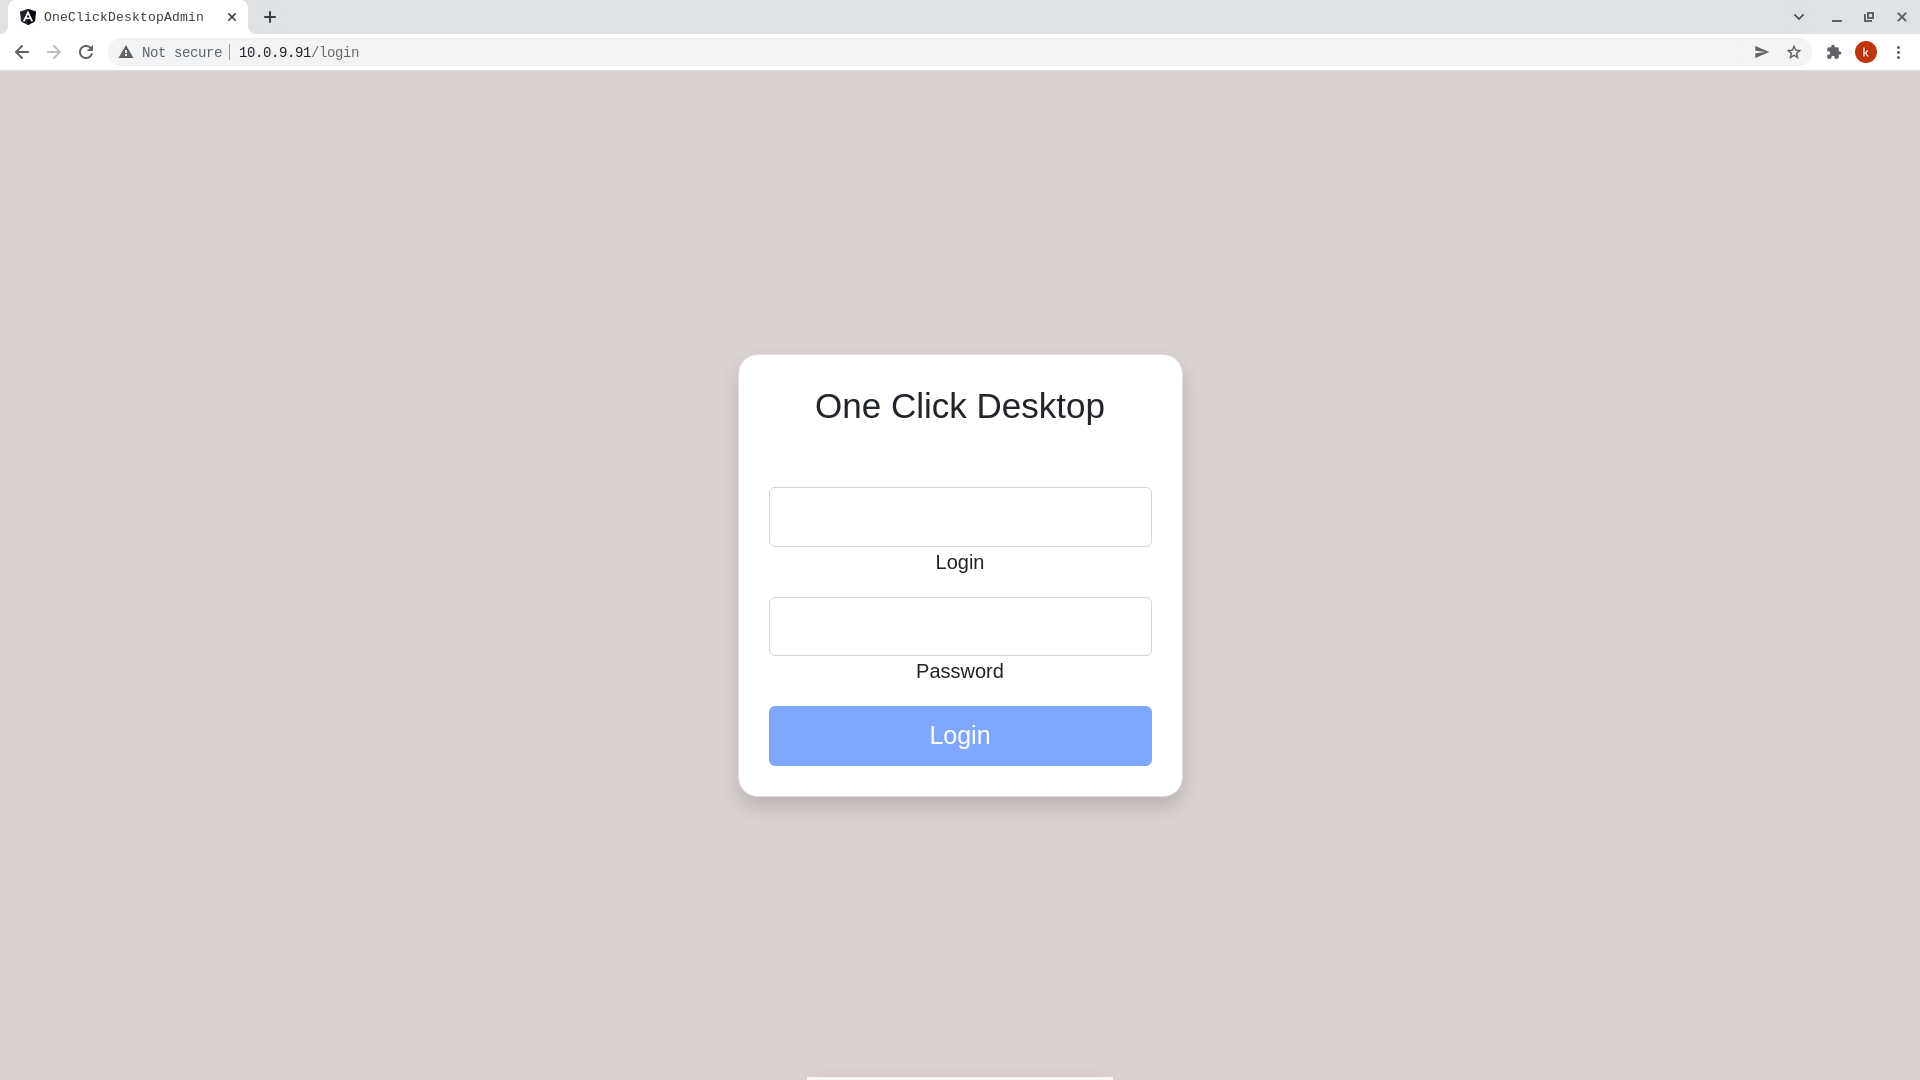
\includegraphics[width=\textwidth]{resources/admin_panel_login.png}
  \caption{Okno logowania panelu administracyjnego}
  \label{figure:system_interaction.admin.login}
\end{figure}

Po zalogowaniu administrator ma dostęp do głównego panelu z podsumowaniem wszystkich dostępnych zasobów.
Po lewej stronie ma on dostępną listę wszystkich aktywnych serwerów wirtualizacji w systemie (rysunek \ref{figure:system_interaction.admin.panel}).

\begin{figure}[ht!]
  \centering
  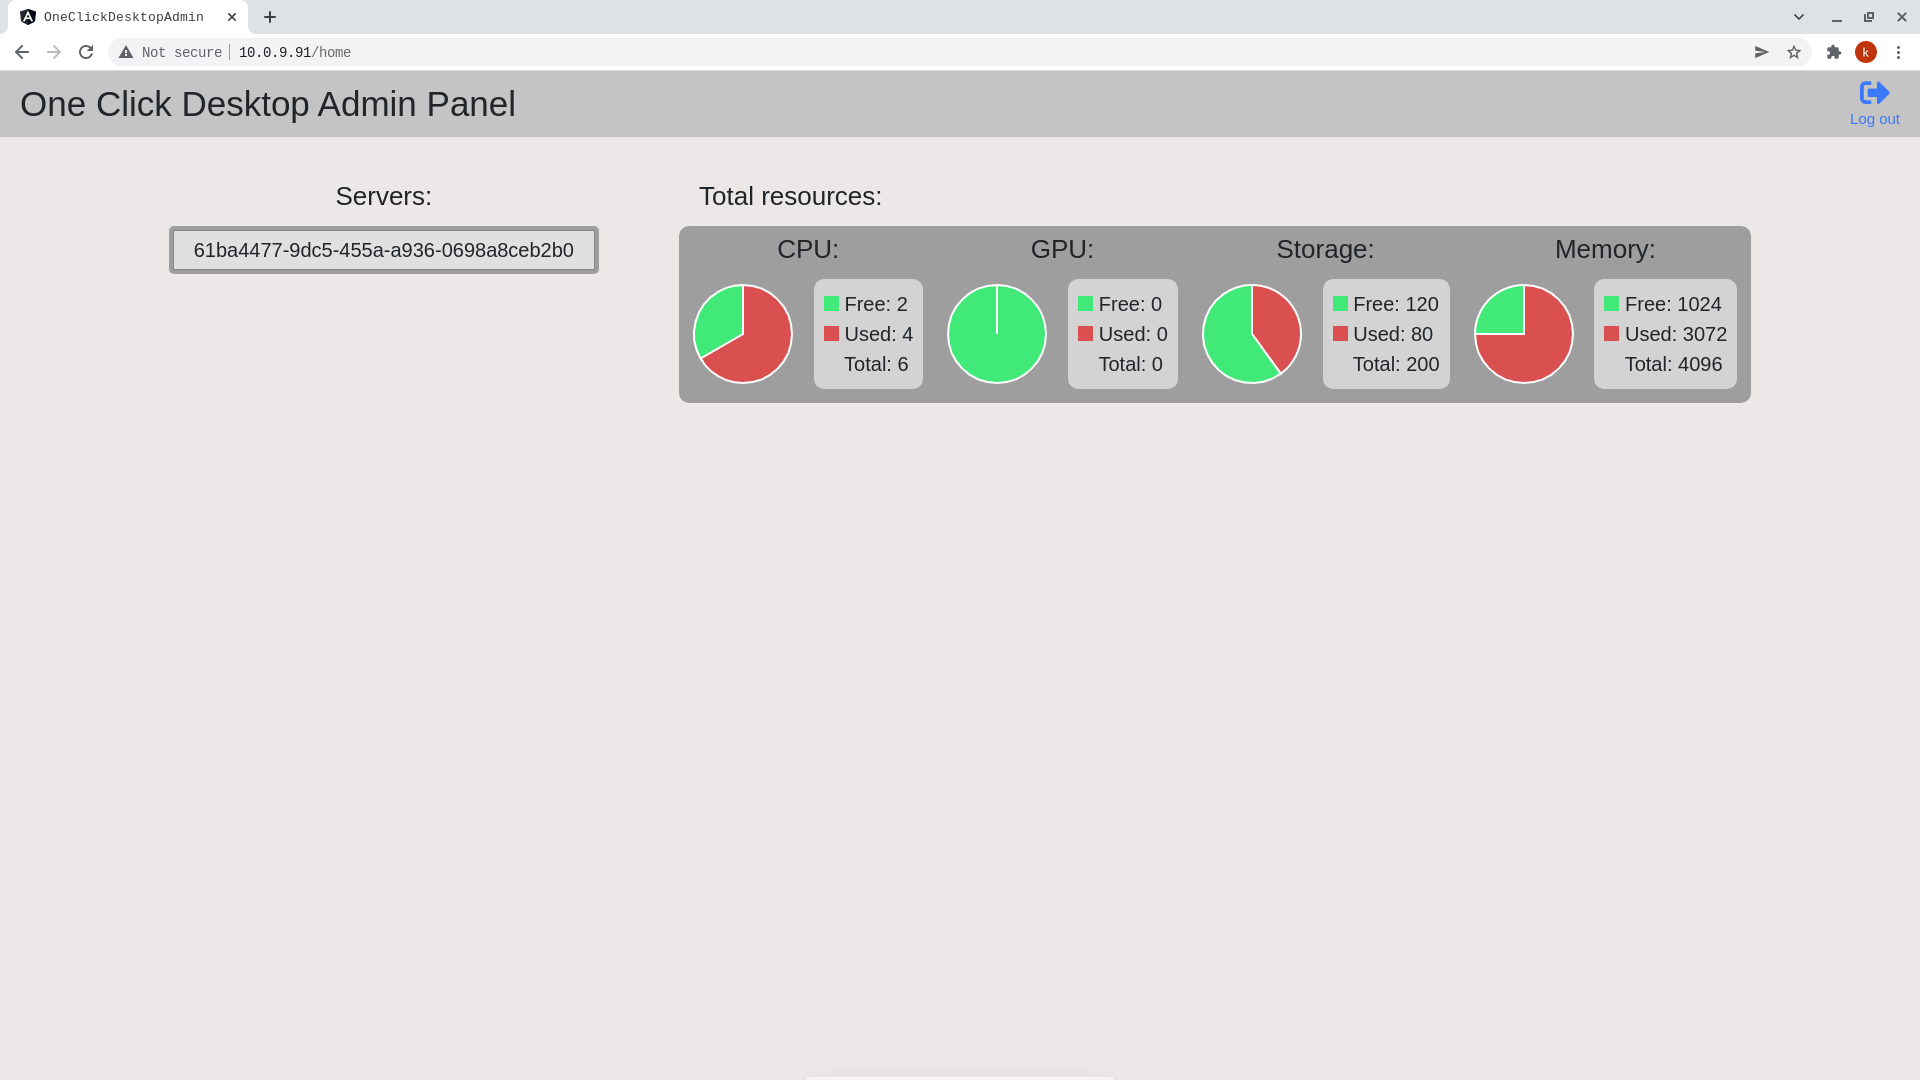
\includegraphics[width=\textwidth]{resources/admin_panel_home.png}
  \caption{Widok wszystkich zasobów systemu}
  \label{figure:system_interaction.admin.panel}
\end{figure}

Po naciśnięciu na wybrany serwer wirtualizacji na środku pojawiają się szczegółowy opis zasobów konkretnego serwera (rysunek \ref{figure:system_interaction.admin.details}).
Administrator, oprócz zasobów, może sprawdzić ile aktualnie jest uruchomionych maszyn (sekcja \textit{Running}) oraz ile jeszcze można uruchomić (sekcja \textit{Free}).

\begin{figure}[ht!]
  \centering
  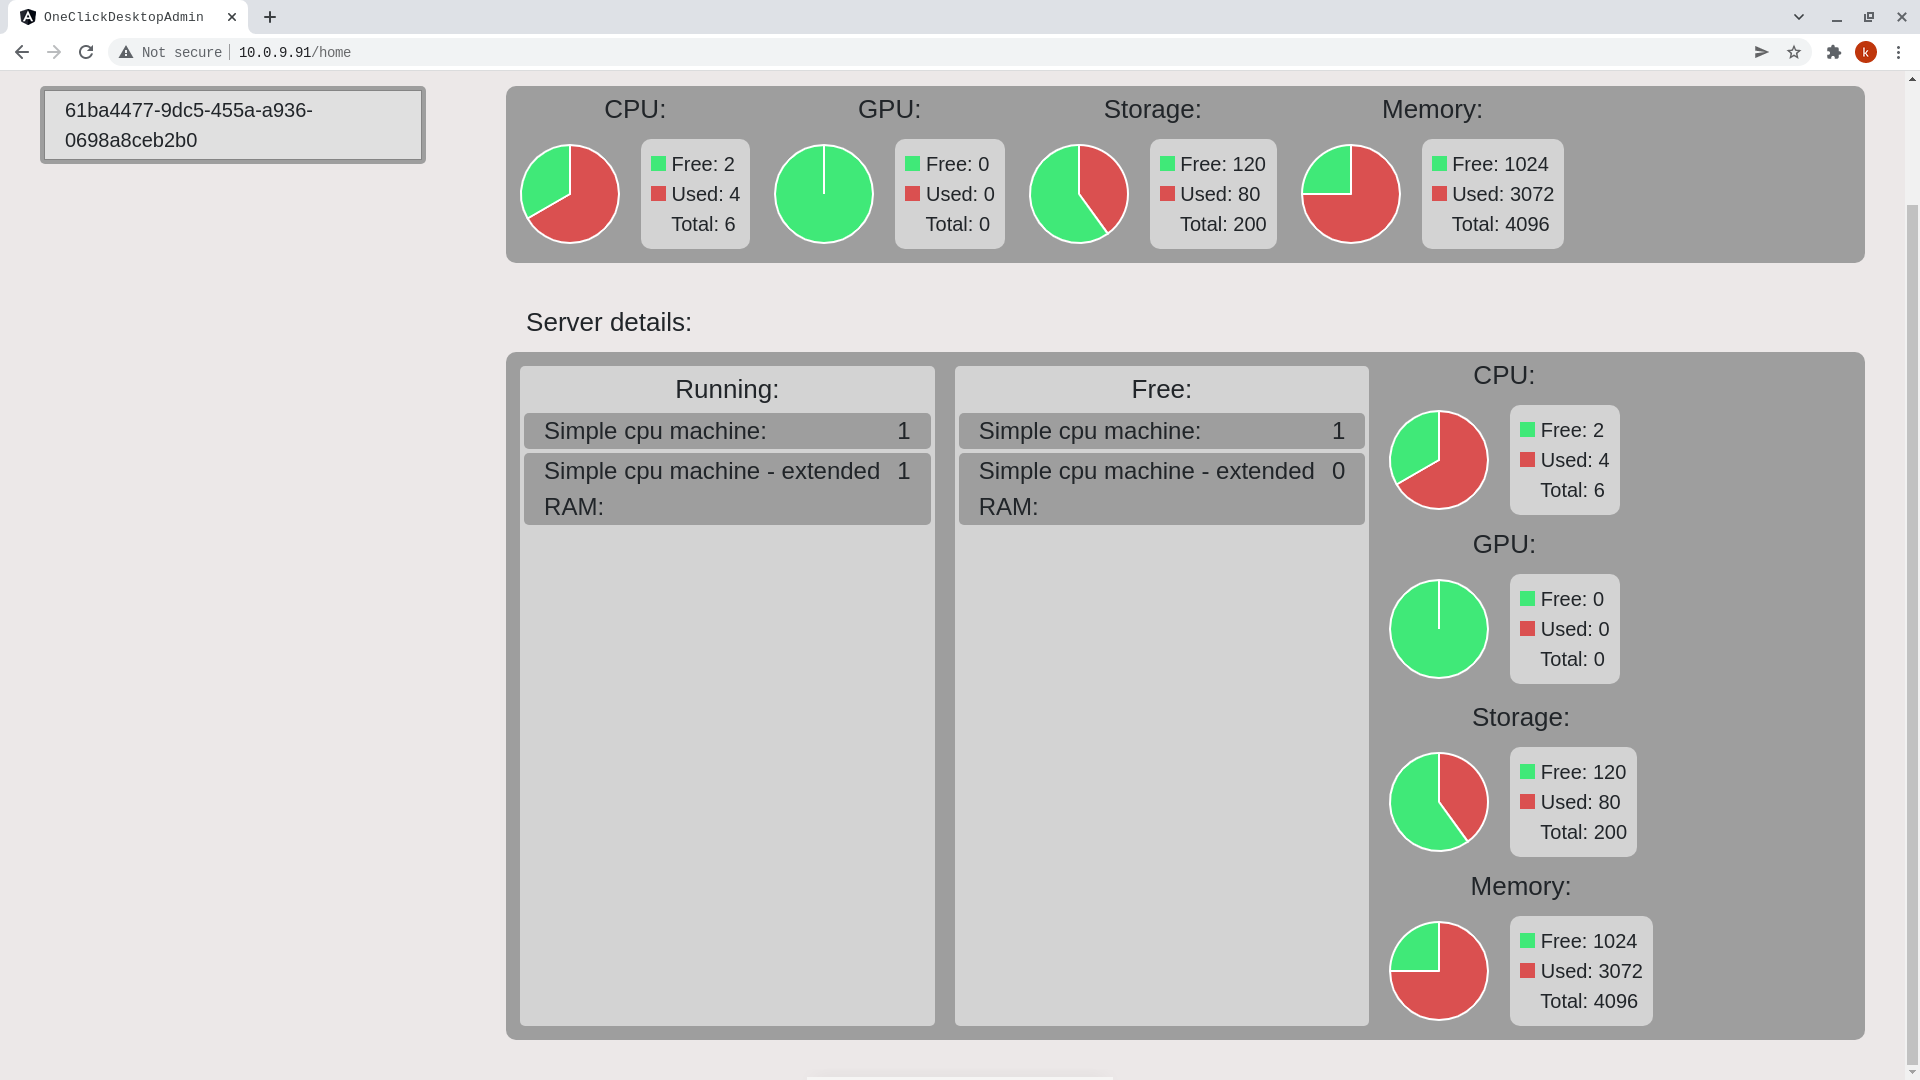
\includegraphics[width=\textwidth]{resources/admin_panel_details.png}
  \caption{Widok szczegółowych zasobów serwera wirtualizacji}
  \label{figure:system_interaction.admin.details}
\end{figure}

Zawartość panelu odświeża się automatycznie.

\newpage
\subsection{Funkcje aplikacji klienckiej}

Po uruchomieniu aplikacji klienckiej użytkownik musi podać nazwę użytkownika i hasło (rysunek \ref{figure:system_interaction.client.login}).
Jeżeli użytkownik istnieje w bazie, to przejdzie do ekranu głównego.
W przeciwnym wypadku zostanie zwrócony błąd dostępu.

\begin{figure}[ht!]
  \centering
  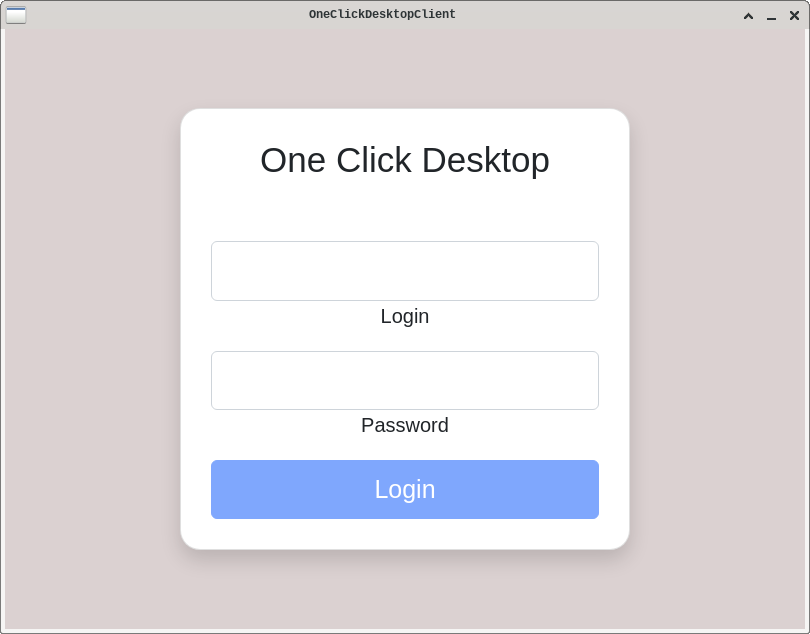
\includegraphics[width=\textwidth]{resources/client_login.png}
  \caption{Ekran logowania aplikacji klienckiej}
  \label{figure:system_interaction.client.login}
\end{figure}

Po zalogowaniu użytkownik trafia do ekranu głównego (rysunek \ref{figure:system_interaction.client.home}).
Może tutaj zobaczyć ile jest dostępnych maszyn w systemie, poprosić o sesję oraz zmienić ustawienia aplikacji.

\begin{figure}[ht!]
  \centering
  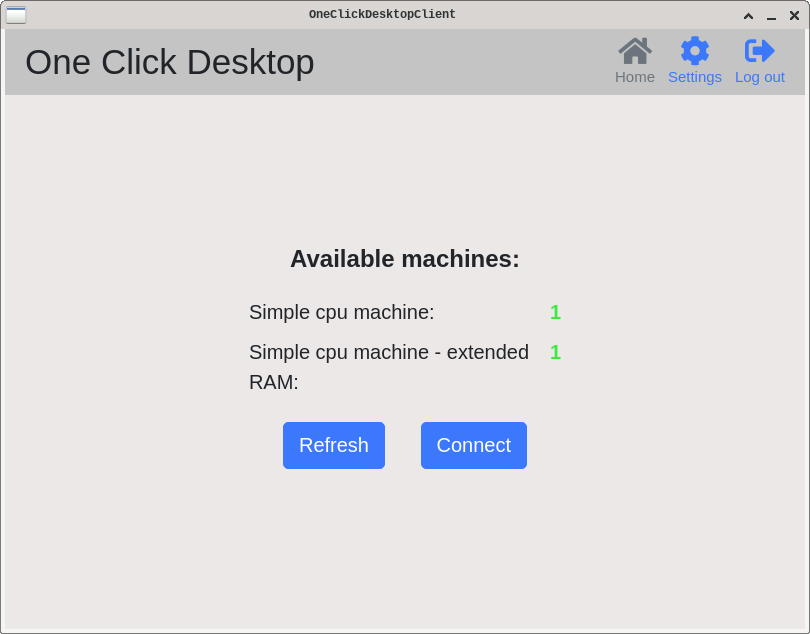
\includegraphics[width=\textwidth]{resources/client_home.png}
  \caption{Ekran główny aplikacji klienckiej}
  \label{figure:system_interaction.client.home}
\end{figure}

Przechodząc do ustawień (rysunek \ref{figure:system_interaction.client.settings}) użytkownik może edytować plik konfiguracyjny z poziomu aplikacji albo wrócić do ekranu głównego.
Zmiana adresu nadzorcy będzie wymagać ponownego uruchomienia.
Inne ustawienia zostaną zastosowane od razu po zmianie.

\begin{figure}[ht!]
  \centering
  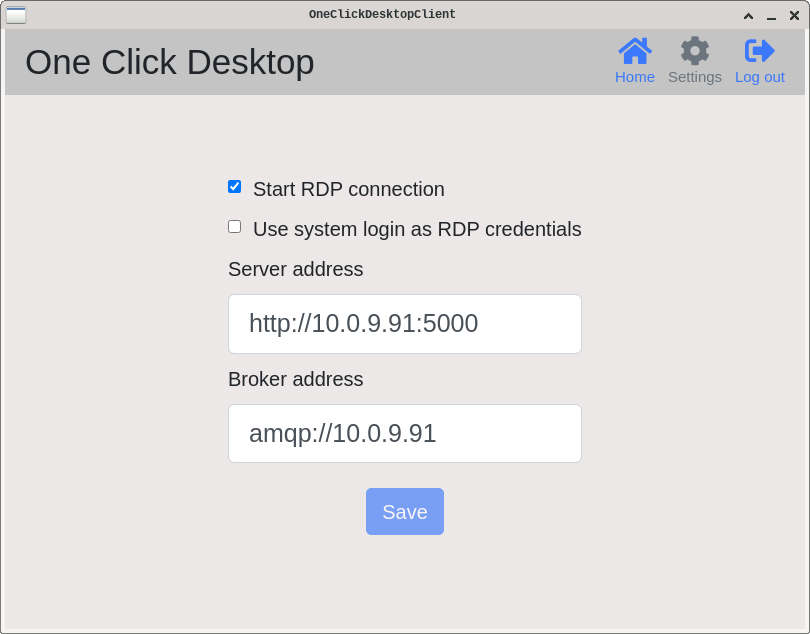
\includegraphics[width=\textwidth]{resources/client_settings.png}
  \caption{Ekran ustawień aplikacji klienckiej}
  \label{figure:system_interaction.client.settings}
\end{figure}

Gdy użytkownik z ekranu głównego naciśnie przycisk \textit{Connect} zostanie zapytany o typ sesji, jaki system ma mu przypisać (rysunek \ref{figure:system_interaction.client.select}).

\begin{figure}[ht!]
  \centering
  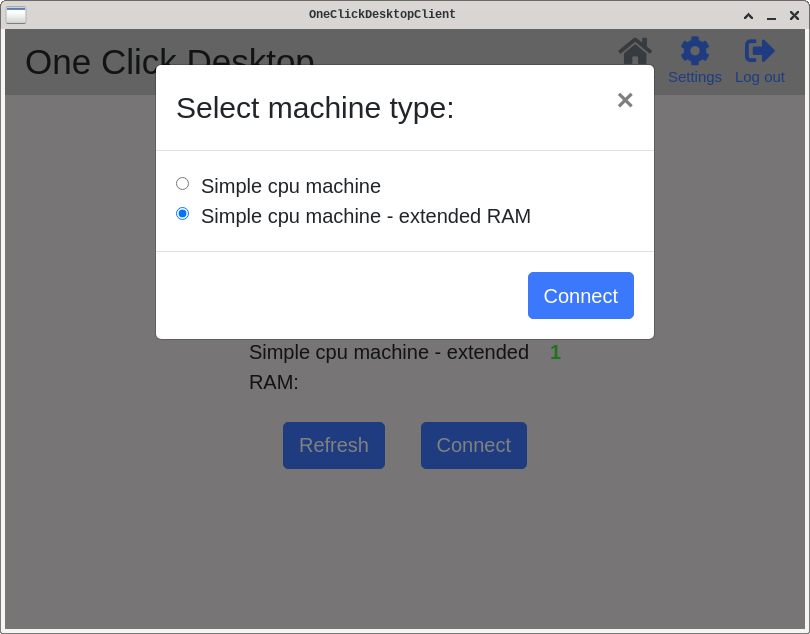
\includegraphics[width=\textwidth]{resources/client_select.png}
  \caption{Ekran wyboru typu maszyny do pracy}
  \label{figure:system_interaction.client.select}
\end{figure}

Po wybraniu jednego z typów sesji i naciśnięciu przycisku \textit{Connect} aplikacja kliencka wyśle prośbę o znalezienie maszyny danego typu i utworzenie sesji dla pytającego użytkownika.
Do czasu utworzenia sesji aplikacja będzie oczekiwać na dane do połączenia.
W przypadku poprawnego utworzenia sesji uruchomi się klient RDP i będzie można rozpocząć pracę.
W przeciwnym wypadku zostanie zgłoszony błąd, a prośba o sesję zostanie umorzona.

Po prawidłowym utworzeniu sesji aplikacja rozpocznie zgłaszanie do zewnętrznego brokera wiadomości, że użytkownik pracuje na maszynie wirtualnej.
Ten stan reprezentuje ekran pokazany na rysunku \ref{figure:system_interaction.client.session}.
Zamknięcie klienta RDP lub naciśniecie przycisku \textit{End session} spowoduje oznaczenie sesji jako \textit{do usunięcia}.
Od tego momentu użytkownik ma \texttt{DomainShutdownTimeout} minut na powrót do swojej sesji (szczegóły w rozdziale \ref{system_startup.overseer_conf}).
Po upływie tego czasu sesja zostaje zamknięta, a maszyna z nią skojarzona wyłączona.

Użytkownik może być podłączony tylko do jednej sesji jednocześnie.
Przy prośbie o sesję typu, dla którego już taka istnieje, system zwróci informację o istniejącej sesji.
Nie może on dostać następnej sesji tego samego typu.
Istnieje jednak możliwość korzystania z dwóch sesji różnych typów w tym samym momencie.
Aby to wykonać należy uruchomić następna aplikacje kliencką, zalogować się do niej tymi samymi danymi dostępowymi oraz poprosić o sesję innego typu niż w przypadku pierwszej aplikacji klienckiej.
Wtedy każda aplikacja kliencka będzie śledzić jeden proces klienta RDP.

Podczas korzystania z maszyny wirtualnej, użytkownik ma dostęp do aplikacji przygotowanych wcześniej przez administratora.
Może na niej zrobić wszystko, jednak tylko zawartość folderu domowego przeniesie się do następnie uruchomionej sesji.
Maszyna po każdej zakończonej sesji zostanie zniszczona.
Jedyne czego nie może zrobić użytkownik: wyłączać maszynę, restartować maszynę, zmieniać ustawienia interfejsów sieciowych.
Spowoduje to niespójność modelu i ostatecznie będzie wymagało restartu wybranych serwerów wirtualizacji. 

\begin{figure}[ht!]
  \centering
  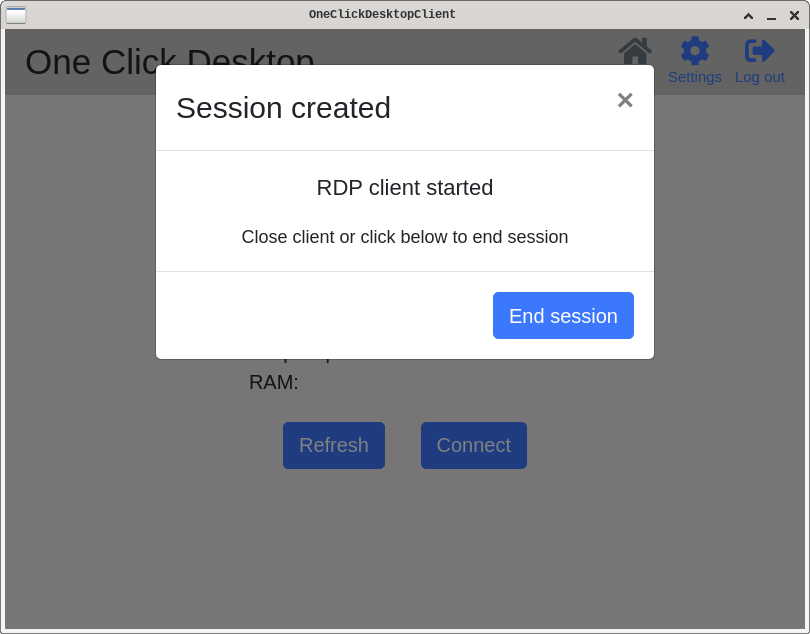
\includegraphics[width=\textwidth]{resources/client_session.png}
  \caption{Ekran działającego połączenia RDP}
  \label{figure:system_interaction.client.session}
\end{figure}

W przypadku gdy użytkownik poprosi aby nie uruchamiać dołączonego klienta RDP, albo uruchomienie klienta RDP zakończy się błędem, zostaną mu przekazane dane dostępowe do przypisanej maszyny wirtualnej (rysunek \ref{figure:system_interaction.client.session_nordp}).
Wtedy jedynym sposobem na zaznaczenie, że skończyło się pracę na maszynie, jest naciśnięcie przycisku \textit{End session}.

\begin{figure}[ht!]
  \centering
  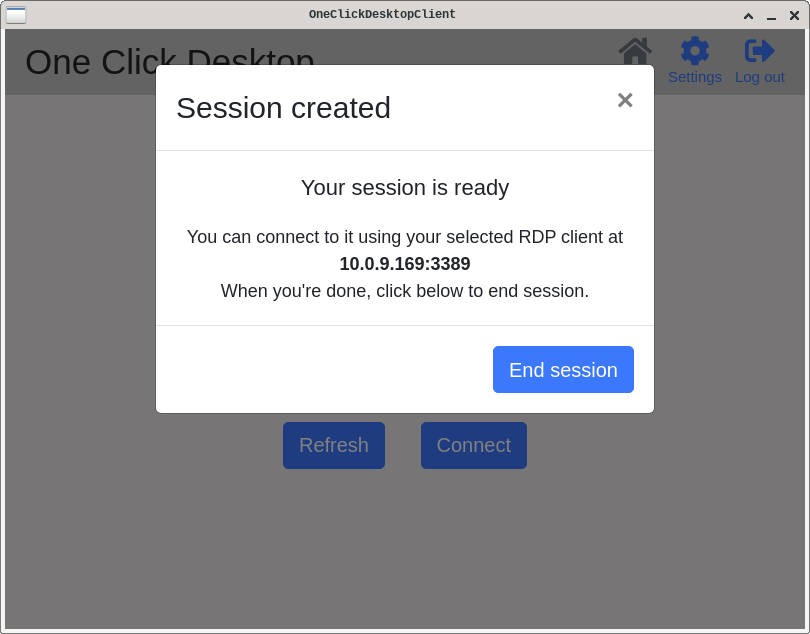
\includegraphics[width=\textwidth]{resources/client_session_nordp.png}
  \caption{Ekran trwania połączenia w zewnętrznym kliencie RDP}
  \label{figure:system_interaction.client.session_nordp}
\end{figure}


\end{document}